\chapter{Evaluación de proyectos de inversión}
\label{cap:inversiones}

\section{Plata hoy no es plata mañana}

Invertir es resignar dinero hoy a cambio de flujos futuros inciertos: comprar una máquina, abrir una sucursal, lanzar un producto. La pregunta de gestión es \emph{¿conviene?}, y para responderla hace falta un principio que parece obvio pero lo cambia todo: \textbf{un peso hoy vale más que un peso dentro de un año}. Por tres razones —puedo invertirlo y ganar interés, la inflación le quita poder de compra, y el futuro es incierto— el dinero tiene \emph{valor tiempo} \cite{brealey}.

\section{Descontar: traer el futuro al presente}

Si la tasa de interés relevante es $r$, un flujo $F$ que se recibe dentro de $t$ años vale hoy:
\begin{equation}
\text{Valor presente} = \frac{F}{(1+r)^{t}}.
\end{equation}
Dividir por $(1+r)^t$ se llama \textbf{descontar}, y $r$ es la \emph{tasa de descuento} (el costo de oportunidad del capital). Descontar permite comparar flujos de distintos momentos en una unidad común: pesos de hoy.

\section{El Valor Actual Neto (VAN)}

\begin{definicion}[Valor Actual Neto]
El \emph{VAN} de un proyecto con flujos $F_0, F_1,\dots,F_n$ es la suma de todos los flujos descontados:
\[
\van = \sum_{t=0}^{n}\frac{F_t}{(1+r)^{t}} = F_0 + \frac{F_1}{(1+r)} + \cdots + \frac{F_n}{(1+r)^{n}},
\]
donde $F_0$ es la inversión inicial (negativa) y no se descuenta porque ocurre en $t=0$.
\end{definicion}

\begin{ideabox}
\textbf{Criterio del VAN.} Si $\van > 0$, el proyecto crea valor (rinde más que la tasa exigida): \emph{conviene}. Si $\van<0$, destruye valor: no conviene. Entre proyectos alternativos, se elige el de mayor VAN. Es el criterio teóricamente más sólido \cite{brealey}.
\end{ideabox}

\section{La Tasa Interna de Retorno (TIR)}

\begin{definicion}[Tasa Interna de Retorno]
La \emph{TIR} es la tasa de descuento que hace el VAN igual a cero:
\[
\sum_{t=0}^{n}\frac{F_t}{(1+\tir)^{t}} = 0 .
\]
\end{definicion}

La TIR es la «rentabilidad propia» del proyecto. El criterio: se acepta si la TIR supera la tasa de corte $r$ (el costo del capital). Para proyectos simples, TIR y VAN dan la misma recomendación; pero la TIR tiene trampas —puede no existir, o haber varias si los flujos cambian de signo más de una vez— por lo que ante conflicto se prioriza el VAN \cite{sapag}.

\section{Refinamientos: TIRM y período de recupero}

\paragraph{TIR modificada (TIRM).} La TIR supone, irrealistamente, que los flujos intermedios se reinvierten a la propia TIR. La \textbf{TIRM} corrige esto distinguiendo una tasa de financiamiento (para los egresos) y una de reinversión (para los ingresos), dando una rentabilidad más realista.

\paragraph{Período de recupero (payback).} Responde «¿en cuánto tiempo recupero la inversión?». El \emph{payback simple} acumula los flujos sin descontar; el \emph{payback descontado} (PRD) acumula los flujos ya descontados, que es lo correcto porque respeta el valor tiempo. Es un criterio de \emph{liquidez/riesgo} complementario al VAN, no un sustituto.

\paragraph{Perfil del VAN.} Es el gráfico del VAN en función de la tasa de descuento. Es una curva decreciente que cruza el eje horizontal exactamente en la TIR: una imagen que reúne ambos criterios en un solo vistazo.

\begin{ejemplo}[¿Compro la máquina?]
Una inversión de \$1000 hoy genera \$400 anuales durante 4 años. La tasa de corte es $r=10\%$.
\[
\van = -1000 + \frac{400}{1.1} + \frac{400}{1.1^2} + \frac{400}{1.1^3} + \frac{400}{1.1^4} \approx -1000 + 1267.95 = 267.95 .
\]
Como $\van \approx \$268 > 0$, el proyecto conviene. La TIR (la tasa que anula el VAN) es $\tir \approx 21.9\%$, bastante mayor que el $10\%$ exigido: misma conclusión por otro camino. El \emph{payback simple} es $1000/400 = 2.5$ años, pero el \emph{descontado} es $\approx 3.0$ años, porque los flujos valen menos al traerlos a hoy.
\end{ejemplo}

\begin{figure}[htbp]
\centering
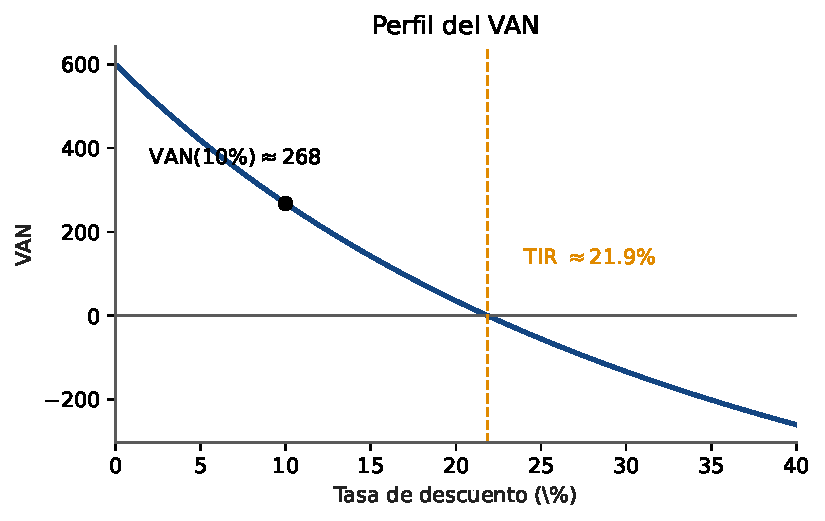
\includegraphics[width=0.72\linewidth]{figuras/van_perfil}
\caption{El perfil del VAN: a mayor tasa de descuento, menor VAN. La curva cruza el cero exactamente en la TIR, uniendo ambos criterios en una sola imagen.}
\label{fig:van_perfil}
\end{figure}

\section{La inversión, en el contexto macro}

¿De dónde sale la tasa de descuento? En buena medida, de las condiciones financieras de la economía. Blanchard~\cite{blanchard} subraya que la inversión agregada depende negativamente de la tasa de interés: tasas más altas encarecen el capital, suben la valla que un proyecto debe superar y, por lo tanto, hay menos proyectos con VAN positivo. Así, la decisión micro de una empresa (este capítulo) y la dinámica macro de la inversión (la macroeconomía) son dos miradas del mismo fenómeno \cite{blanchard}.

\begin{labbox}
La librería \texttt{numpy\_financial} implementa estos criterios directamente: \texttt{npv(tasa, flujos)} para el VAN, \texttt{irr(flujos)} para la TIR y \texttt{mirr(...)} para la TIRM. El payback descontado se calcula a mano, acumulando los flujos descontados hasta que el acumulado cruza cero. Y el perfil del VAN es, simplemente, evaluar \texttt{npv} para una lista de tasas y graficar: la curva corta el eje en la TIR, uniendo en una figura toda la teoría del capítulo.
\end{labbox}

\section{Síntesis del capítulo}

El valor tiempo del dinero obliga a descontar los flujos futuros. El VAN —crear o destruir valor— es el criterio rey; la TIR, el payback y la TIRM lo complementan desde la rentabilidad y la liquidez. Con esto cerramos el recorrido económico del curso: del precio de un bien a la decisión de invertir, todo el camino se apoya en las mismas funciones, derivadas, integrales y sistemas que vimos.
